Word2Vec \cite{w2v} è un algoritmo di apprendimento automatico fondamentale nel campo del Trattamento del Linguaggio Naturale (Natural Language Processing, NLP). Introdotta da Mikolov et al. nel 2013, questa tecnica ha segnato una svolta nel modo in cui le parole vengono rappresentate come vettori numerici e come sono comprese le relazioni semantiche tra di loro. L'obiettivo principale di Word2Vec è di catturare la somiglianza semantica tra le parole, consentendo alle macchine di elaborare il linguaggio in modo significativo.

\subsubsection{La logica dietro Word2Vec}
Word2Vec sfrutta il principio di distribuzione del linguaggio naturale, che afferma che parole simili tendono a comparire nei medesimi contesti. L'algoritmo considera il contesto in cui le parole compaiono in un testo e cerca di rappresentare ogni parola in base al suo contesto di utilizzo. Questo processo cattura le relazioni semantiche tra le parole: parole simili avranno rappresentazioni simili.

\subsubsection{Continuous Bag of Words (CBOW) e Skip-gram}
Word2Vec offre due approcci principali: Continuous Bag of Words (CBOW) e Skip-gram. Nel modello CBOW, l'algoritmo cerca di prevedere una parola data una finestra di contesto, utilizzando il contesto per stimare la parola obiettivo. Nel modello Skip-gram, invece, l'obiettivo è prevedere il contesto (cioè le parole circostanti) data una parola. Entrambi gli approcci cercano di ottimizzare la capacità dell'algoritmo di rappresentare le parole in modo accurato.
Nella figura \ref{fig:cbow} è possibile osservare un esempio di modello CBOW, mentre nella figura \ref{fig:skipgram} è possibile osservare un esempio di modello Skip-gram.
\begin{center}
    \begin{figure}[H]
        \centering
        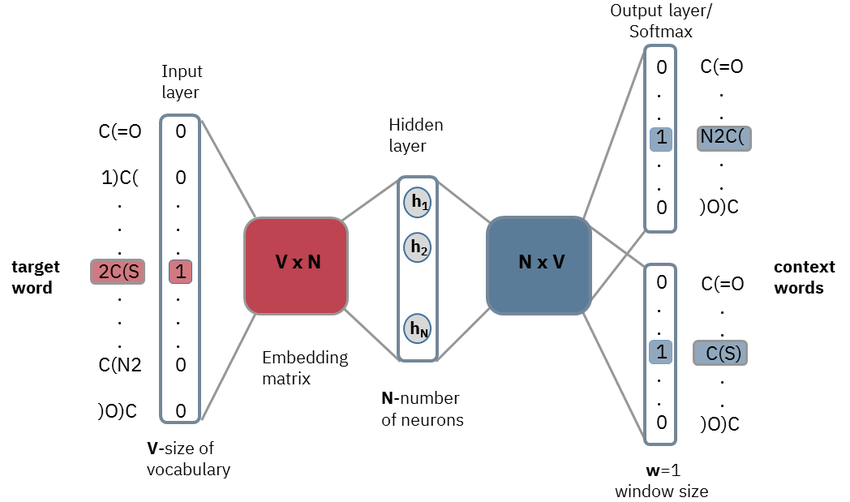
\includegraphics[width=0.7\pdfpagewidth]{images/skipgram.jpg}
        \caption{Esempio di modello Skip-gram}
        \label{fig:skipgram}
    \end{figure}
\end{center}

\begin{center}
    \begin{figure}[H]
        \centering
        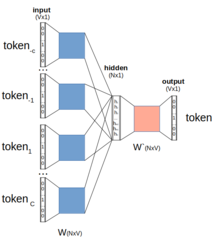
\includegraphics{images/CBOW.png}
        \caption{Esempio di modello Continous Bag of Words (CBOW)}
        \label{fig:cbow}
    \end{figure}
\end{center}

\subsubsection{Addestramento e ottimizzazione}
Durante la fase di addestramento di Word2Vec, l'algoritmo cerca di regolare i parametri in modo che i vettori delle parole riflettano le relazioni semantiche. Questo avviene attraverso l'ottimizzazione di una funzione obiettivo che misura la discrepanza tra le parole reali e quelle previste. L'addestramento avviene attraverso iterazioni multiple su un grande corpus di testi, affinando gradualmente i vettori delle parole.

\subsubsection{Vantaggi e sfide}
Word2Vec ha introdotto importanti vantaggi nel campo del NLP, rendendo possibile la rappresentazione numerica del linguaggio. Questi vettori di parole sono state sfruttati con successo in varie applicazioni NLP, migliorando la comprensione del contesto e la similarità semantica tra le parole. Tuttavia, Word2Vec presenta sfide, come la gestione di parole polisemiche e la cattura di sfumature linguistiche complesse.

\subsubsection{Eredità e avanzamenti successivi}
L'eredità di Word2Vec risiede nell'apertura della strada all'uso di rappresentazioni vettoriali per il linguaggio naturale. L'algoritmo ha ispirato ulteriori sviluppi, come GloVe e i modelli Transformer, che hanno ulteriormente migliorato le prestazioni nell'elaborazione del linguaggio.
